% Vietnamese translation for OI Public Library
% Source-PDF: 英文资料 ENGLISH MATERIALS/Game Theory - Thomas S. Ferguson.pdf
\documentclass[11pt]{article}
\usepackage{oipl-vn}
\usepackage{graphicx}
\usepackage{tikz}

\newcommand{\SG}{\operatorname{SG}}
\newcommand{\mex}{\operatorname{mex}}
\newcommand{\xor}{\mathbin{\oplus}}
\newcommand{\nimprod}{\mathbin{\otimes}}

\newcommand{\FergusonNimbleFigure}{%
\begin{center}
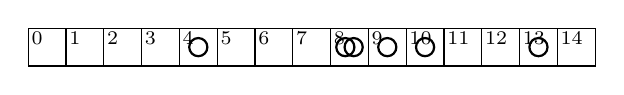
\begin{tikzpicture}[x=0.48cm,y=0.48cm,every node/.style={font=\scriptsize}]
  \draw (0,0) rectangle (15,1);
  \foreach \x in {1,...,14} \draw (\x,0)--(\x,1);
  \foreach \x in {0,...,14} \node[anchor=north west,inner sep=1pt] at (\x,1) {\x};
  \foreach \x/\dx in {4/0,8/-0.11,8/0.11,9/0,10/0,13/0}
    \draw[thick] (\x+0.5+\dx,0.5) circle (0.24);
\end{tikzpicture}\\[-0.2em]
{\small Vị trí Nimble: sáu xu ở các ô \(4,8,8,9,10,13\).}
\end{center}
}

\newcommand{\FergusonNorthcottFigure}{%
\begin{center}
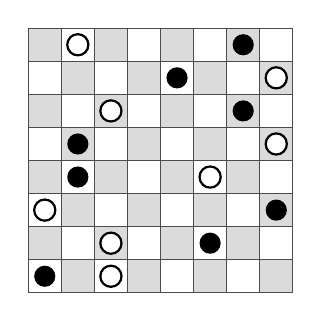
\begin{tikzpicture}[x=0.42cm,y=0.42cm]
  \foreach \r in {0,...,7} {
    \foreach \c in {0,...,7} {
      \pgfmathtruncatemacro{\shade}{mod(\r+\c,2)}
      \ifnum\shade=0
        \fill[gray!28] (\c,7-\r) rectangle +(1,1);
      \fi
      \draw[black!70] (\c,7-\r) rectangle +(1,1);
    }
  }
  \foreach \r/\c in {1/2,2/8,3/3,4/8,5/6,6/1,7/3,8/3}
    \draw[fill=white,thick] (\c-0.5,8.5-\r) circle (0.32);
  \foreach \r/\c in {1/7,2/5,3/7,4/2,5/2,6/8,7/6,8/1}
    \fill[black] (\c-0.5,8.5-\r) circle (0.32);
\end{tikzpicture}\\[-0.2em]
{\small Vị trí Northcott: mỗi hàng có một quân trắng và một quân đen.}
\end{center}
}

\newcommand{\FergusonTwoDimNimFigure}{%
\begin{center}
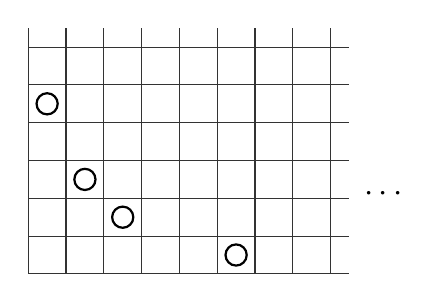
\begin{tikzpicture}[x=0.48cm,y=0.48cm]
  \foreach \x in {0,...,8} \draw[black!80] (\x,0)--(\x,6.5);
  \foreach \y in {0,...,6} \draw[black!80] (0,\y)--(8.5,\y);
  \foreach \x/\y in {0/4,1/2,2/1,5/0}
    \draw[thick] (\x+0.5,\y+0.5) circle (0.28);
  \node[font=\large] at (9.4,2.1) {\(\cdots\)};
\end{tikzpicture}\\[-0.2em]
{\small Vị trí trong Nim hai chiều.}
\end{center}
}

\title{Trò Chơi Tổ Hợp Công Bằng}
\author{Thomas S. Ferguson}
\date{}

\begin{document}
\maketitle

\origtitle{Game Theory, Part I: Impartial Combinatorial Games}
\sourcepath{English Materials/Game Theory - Thomas S. Ferguson.pdf}

\section{Trò chơi lấy quân}

Trò chơi tổ hợp là trò chơi hai người, thông tin hoàn hảo, không có yếu tố ngẫu
nhiên, và kết quả là thắng hoặc thua. Một trò chơi được mô tả bởi tập các vị
trí, một vị trí ban đầu, và người đến lượt đi. Người chơi di chuyển từ vị trí
này sang vị trí khác, thường là luân phiên, cho đến khi đạt một vị trí kết
thúc, tức vị trí không còn nước đi hợp lệ. Khi đó một người được tuyên bố
thắng và người còn lại thua.

Trong phần này ta chỉ xét \term{trò chơi công bằng} dưới luật chơi chuẩn: ở
mỗi vị trí, hai người chơi có cùng tập nước đi hợp lệ, và người đi nước cuối
cùng thắng. Những trò chơi như cờ vua là trò chơi thiên vị vì hai bên điều
khiển các quân khác nhau.

\subsection{Một trò chơi lấy quân đơn giản}

Xét trò chơi sau. Có một đống \(21\) quân. Mỗi lượt một người lấy \(1\), \(2\),
hoặc \(3\) quân. Hai người luân phiên, người thứ nhất đi trước, và người lấy
quân cuối cùng thắng.

Ta phân tích ngược từ cuối ván. Nếu còn \(1\), \(2\), hoặc \(3\) quân, người
đến lượt thắng ngay bằng cách lấy hết. Nếu còn \(4\) quân, người đến lượt buộc
phải để lại \(1\), \(2\), hoặc \(3\) quân, nên đối thủ thắng. Do đó \(4\) là
vị trí thua cho người đến lượt. Tương tự, \(5\), \(6\), \(7\) là vị trí thắng
vì có thể đi về \(4\), còn \(8\) là vị trí thua.

Vì vậy các vị trí mục tiêu là
\[
  0,4,8,12,16,\ldots
\]
tức các số chia hết cho \(4\). Với \(21\) quân, người đi trước thắng bằng nước
duy nhất tối ưu: lấy \(1\) quân và để lại \(20\).

\subsection{Định nghĩa trò chơi tổ hợp}

Một trò chơi tổ hợp trong phạm vi bài này thỏa các điều kiện sau.
\begin{enumerate}
  \item Có hai người chơi.
  \item Có một tập, thường hữu hạn, các vị trí có thể có.
  \item Luật chơi xác định từ mỗi vị trí có thể đi đến những vị trí nào. Nếu
  hai người có cùng lựa chọn tại mọi vị trí, trò chơi là công bằng; ngược lại
  là thiên vị.
  \item Hai người chơi luân phiên đi.
  \item Trò chơi kết thúc khi người đến lượt đứng tại vị trí không có nước đi.
  Với luật chuẩn, người đi nước cuối thắng; với luật \term{misere}, người đi
  nước cuối thua.
  \item Trò chơi kết thúc sau hữu hạn nước đi bất kể hai bên chơi thế nào. Đây
  là \term{điều kiện kết thúc}.
\end{enumerate}

Định nghĩa này loại bỏ xúc xắc, chia bài, nước đi đồng thời, thông tin ẩn, và
các kết quả hòa hữu hạn.

\subsection{Vị trí P và vị trí N}

Một \term{vị trí P} là vị trí thắng cho người vừa đi trước đó
(\textit{previous player}) nếu hai bên chơi tối ưu. Một \term{vị trí N} là vị
trí thắng cho người đến lượt đi (\textit{next player}). Trong trò chơi lấy
\(1\), \(2\), hoặc \(3\) quân ở trên, các vị trí P chính là các bội của \(4\).

Với trò chơi công bằng thỏa điều kiện kết thúc, các vị trí P và N có thể được
gán nhãn bằng quy trình truy hồi sau.
\begin{enumerate}
  \item Mọi vị trí kết thúc được gán nhãn P.
  \item Mọi vị trí đi được trong một nước tới một vị trí P đã gán nhãn được
  gán nhãn N.
  \item Mọi vị trí mà tất cả nước đi đều tới các vị trí N đã gán nhãn được gán
  nhãn P.
  \item Nếu bước trước không tìm thêm vị trí P thì dừng; nếu không, quay lại
  bước 2.
\end{enumerate}

\paragraph{Tính chất đặc trưng.}
Dưới luật chuẩn, các vị trí P và N được xác định bởi ba mệnh đề:
\begin{enumerate}
  \item Mọi vị trí kết thúc là vị trí P.
  \item Từ mỗi vị trí N có ít nhất một nước đi tới vị trí P.
  \item Từ mỗi vị trí P, mọi nước đi đều tới vị trí N.
\end{enumerate}
Chiến lược thắng là luôn đi về vị trí P. Với luật misere, mệnh đề đầu tiên
được thay bằng: mọi vị trí kết thúc là vị trí N.

\subsection{Trò chơi trừ}

Cho \(S\) là một tập các số nguyên dương. \term{Trò chơi trừ} với tập trừ
\(S\) có một đống \(n\) quân; mỗi lượt người chơi lấy \(s\) quân với
\(s\in S\), miễn là còn đủ quân. Người đi nước cuối thắng.

Trò chơi lấy \(1\), \(2\), \(3\) quân là trường hợp \(S=\{1,2,3\}\). Một ví dụ
khác là \(S=\{1,3,4\}\). Ta tìm vị trí P như sau. Vị trí \(0\) là P. Các vị
trí \(1\), \(3\), \(4\) là N vì đi được về \(0\). Vị trí \(2\) là P vì chỉ đi
được về \(1\). Khi tiếp tục, ta nhận được chu kỳ:
\[
\begin{array}{c|ccccccccccccccc}
x&0&1&2&3&4&5&6&7&8&9&10&11&12&13&14\\ \hline
\text{loại}&P&N&P&N&N&N&N&P&N&P&N&N&N&N&P
\end{array}
\]
Mẫu \(P,N,P,N,N,N,N\) có độ dài \(7\) lặp mãi. Do đó các vị trí P là các số
có phần dư \(0\) hoặc \(2\) modulo \(7\). Chẳng hạn \(100\equiv2\pmod 7\), nên
với \(100\) quân, người đi sau thắng nếu chơi tối ưu.

Các bài tập trong bản gốc mở rộng phần này sang luật misere, trò chơi số \(31\),
Chomp, trò chơi trừ động, Fibonacci Nim và trò SOS; chúng dùng cùng ý tưởng gán
nhãn P/N nhưng không cần thiết cho phần lý thuyết chính dưới đây.

\section{Trò chơi Nim}

Nim là trò chơi lấy quân nổi tiếng nhất. Có các đống quân kích thước
\(x_1,x_2,\ldots,x_n\). Mỗi lượt chọn đúng một đống và lấy khỏi đó một số quân
dương tùy ý, có thể lấy cả đống. Người lấy quân cuối cùng thắng.

\subsection{Phân tích ban đầu}

Vị trí kết thúc duy nhất là \((0,0,\ldots,0)\), nên đó là vị trí P. Với một
đống khác rỗng, người đến lượt thắng bằng cách lấy hết đống đó. Với hai đống,
các vị trí P là những vị trí có hai đống bằng nhau: \((a,a)\). Nếu đối thủ làm
hai đống khác nhau, ta lấy ở đống lớn để đưa về hai đống bằng nhau.

Với ba đống, mẫu hình không còn hiển nhiên. Các vị trí nhỏ như
\((1,1,1)\), \((1,1,2)\), \((1,1,3)\), \((1,2,2)\) đều là N, còn
\((1,2,3)\) là P. Các vị trí P tiếp theo gồm \((1,4,5)\) và \((2,4,6)\). Quy
luật tổng quát được mô tả bằng tổng Nim.

\subsection{Tổng Nim}

Viết các số không âm ở hệ nhị phân. \term{Tổng Nim} của hai số là phép cộng
từng bit modulo \(2\), tức phép xor bit. Ta ký hiệu bằng \(\xor\).

\paragraph{Định nghĩa.}
Nếu
\[
  x=(x_mx_{m-1}\ldots x_0)_2,\qquad
  y=(y_my_{m-1}\ldots y_0)_2,
\]
thì
\[
  x\xor y=(z_mz_{m-1}\ldots z_0)_2,\qquad
  z_k\equiv x_k+y_k\pmod 2.
\]
Ví dụ:
\[
\begin{array}{rcl}
22&=&10110_2,\\
51&=&110011_2,\\ \hline
22\xor 51&=&100101_2=37.
\end{array}
\]

Phép \(\xor\) giao hoán, kết hợp, có phần tử đơn vị \(0\), và mỗi số là nghịch
đảo của chính nó: \(x\xor x=0\). Do đó luật khử đúng:
\[
  x\xor y=x\xor z \quad\Longrightarrow\quad y=z.
\]

\paragraph{Định lý Bouton.}
Một vị trí Nim \((x_1,x_2,\ldots,x_n)\) là vị trí P khi và chỉ khi
\[
  x_1\xor x_2\xor\cdots\xor x_n=0.
\]

Ví dụ, với \((13,12,8)\),
\[
\begin{array}{rcl}
13&=&1101_2,\\
12&=&1100_2,\\
8&=&1000_2,\\ \hline
13\xor12\xor8&=&1001_2=9.
\end{array}
\]
Vì tổng Nim khác \(0\), đây là vị trí N. Một nước thắng là đổi \(13\) thành
\(4\), tức lấy \(9\) quân ở đống \(13\):
\[
  4\xor12\xor8=0.
\]
Một nước thắng khác là đổi \(12\) thành \(5\).

\subsection{Chứng minh định lý Bouton}

Gọi \(\mathcal P\) là tập các vị trí Nim có tổng Nim bằng \(0\), và
\(\mathcal N\) là phần bù.

Trước hết, vị trí kết thúc thuộc \(\mathcal P\) vì \(0\xor0\xor\cdots=0\).

Tiếp theo, từ mỗi vị trí thuộc \(\mathcal N\), luôn có nước đi về
\(\mathcal P\). Hãy viết tổng Nim theo từng cột bit, và xét cột trái nhất có
số bit \(1\) lẻ. Chọn một đống có bit \(1\) ở cột đó, rồi giảm kích thước đống
ấy sao cho sau khi thay đổi, mọi cột đều có số bit \(1\) chẵn. Số mới nhỏ hơn
số cũ vì bit có trọng số lớn nhất đang xét đổi từ \(1\) thành \(0\), nên đây
là nước đi hợp lệ.

Cuối cùng, không có nước nào từ \(\mathcal P\) về \(\mathcal P\). Nếu chỉ một
đống \(x_1\) được đổi thành \(x'_1<x_1\), thì việc
\[
  x_1\xor x_2\xor\cdots=0=x'_1\xor x_2\xor\cdots
\]
sẽ kéo theo \(x_1=x'_1\) bởi luật khử, mâu thuẫn. Ba tính chất đặc trưng của
vị trí P/N chứng minh định lý.

Từ phần xây dựng trên, số nước thắng từ một vị trí N bằng số bit \(1\) trong
cột trái nhất có tổng lẻ; do đó số nước thắng luôn là số lẻ.

\subsection{Nim misere}

Với Nim misere, người lấy quân cuối cùng thua. Cách chơi tối ưu của Bouton là:
chơi như Nim chuẩn chừng nào còn ít nhất hai đống có kích thước lớn hơn \(1\).
Khi đối thủ đi để chỉ còn đúng một đống có kích thước lớn hơn \(1\), hãy giảm
đống đó về \(0\) hoặc \(1\) sao cho số đống kích thước \(1\) còn lại là số lẻ.

Lý do là trong phần Nim chuẩn, nước tối ưu không bao giờ buộc ta để lại đúng
một đống lớn hơn \(1\) nếu đang ở vị trí cần đưa tổng Nim về \(0\). Khi ván cờ
rơi vào pha chỉ gồm các đống \(1\) và nhiều nhất một đống lớn, điều kiện thắng
của luật misere chỉ còn là chẵn lẻ của số đống \(1\).

\section{Trò chơi trên đồ thị}

Mọi trò chơi tổ hợp công bằng có thể được biểu diễn bằng một đồ thị có hướng:
vị trí là đỉnh, và nước đi là cạnh có hướng. Cách nhìn này dẫn đến hàm
Sprague--Grundy.

\subsection{Đồ thị trò chơi}

\paragraph{Định nghĩa.}
Một đồ thị có hướng là cặp \(G=(X,F)\), trong đó \(X\) là tập đỉnh khác rỗng
và \(F\) là hàm gán cho mỗi \(x\in X\) một tập con \(F(x)\subset X\). Các phần
tử của \(F(x)\) được gọi là \term{hậu vị} của \(x\). Nếu \(F(x)=\varnothing\),
thì \(x\) là vị trí kết thúc.

Trò chơi trên \(G\) bắt đầu ở \(x_0\). Hai người luân phiên; tại \(x\), người
đến lượt chọn một \(y\in F(x)\). Ai gặp vị trí kết thúc khi đến lượt thì thua.

Ta thường giả sử đồ thị \term{bị chặn tiến triển}: với mọi điểm bắt đầu
\(x_0\), có một số \(n\) sao cho mọi đường đi bắt đầu từ \(x_0\) có độ dài
không quá \(n\). Nếu \(X\) hữu hạn, điều này tương đương với không có chu trình.

Ví dụ, trò chơi trừ với \(S=\{1,2,3\}\) và đống ban đầu \(n\) có
\[
  X=\{0,1,\ldots,n\},\qquad F(0)=\varnothing,
\]
\[
  F(1)=\{0\},\qquad F(2)=\{0,1\},\qquad
  F(k)=\{k-3,k-2,k-1\}\quad(k\ge3).
\]
Có thể đọc đồ thị này như một đường thẳng
\(0,1,\ldots,n\), trong đó mỗi đỉnh \(k\) có cung đi lùi một, hai, hoặc ba
bước nếu hợp lệ.

\subsection{Hàm Sprague--Grundy}

\paragraph{Định nghĩa.}
Hàm Sprague--Grundy của đồ thị \(G=(X,F)\) là hàm \(g:X\to\mathbb N\) thỏa
\[
  g(x)=\min\{n\ge0:\ n\ne g(y)\ \text{với mọi }y\in F(x)\}.
\]
Nếu đặt
\[
  \mex(A)=\text{số nguyên không âm nhỏ nhất không thuộc }A,
\]
thì định nghĩa viết gọn là
\[
  g(x)=\mex\{g(y):y\in F(x)\}.
\]

Với đỉnh kết thúc, tập hậu vị rỗng nên \(g(x)=0\). Với đỉnh mà mọi hậu vị đều
kết thúc, \(g(x)=1\). Trên đồ thị bị chặn tiến triển, định nghĩa truy hồi này
luôn xác định duy nhất một hàm hữu hạn.

Hàm SG giải quyết bài toán thắng thua:
\[
  x\text{ là vị trí P}\quad\Longleftrightarrow\quad g(x)=0.
\]
Nếu \(g(x)>0\), định nghĩa của \(\mex\) bảo đảm tồn tại hậu vị \(y\) với
\(g(y)=0\), nên người chơi có thể đi về vị trí P. Nếu \(g(x)=0\), không hậu vị
nào có giá trị \(0\).

\subsection{Ví dụ}

Với trò chơi trừ \(S=\{1,2,3\}\), ta có
\[
\begin{array}{c|ccccccccccccccc}
x&0&1&2&3&4&5&6&7&8&9&10&11&12&13&14\\ \hline
g(x)&0&1&2&3&0&1&2&3&0&1&2&3&0&1&2
\end{array}
\]
nên nói chung \(g(x)\equiv x\pmod4\).

Trong trò chơi một đống mà mỗi lượt phải lấy ít nhất một nửa số quân hiện có,
ta tính được
\[
\begin{array}{c|ccccccccccccc}
x&0&1&2&3&4&5&6&7&8&9&10&11&12\\ \hline
g(x)&0&1&2&2&3&3&3&3&4&4&4&4&4
\end{array}
\]
tức
\[
  g(x)=\min\{k:2^k>x\}.
\]
Một đống riêng lẻ của trò này rất dễ thắng bằng cách lấy hết, nhưng giá trị SG
trở nên hữu ích khi cộng nhiều đống với nhau.

\subsection{Đồ thị tổng quát hơn}

Nếu chỉ yêu cầu mọi đường đi là hữu hạn, nhưng không có cận chung theo từng
đỉnh bắt đầu, ta có đồ thị \term{hữu hạn tiến triển}. Lúc này lý thuyết SG vẫn
có thể mở rộng bằng quy nạp siêu hạn; giá trị SG có thể là các ordinal như
\(\omega,\omega+1,\omega^2\). Trong các ứng dụng thuật toán thông thường, ta
thường chỉ cần đồ thị hữu hạn không chu trình hoặc đồ thị bị chặn tiến triển.

Nếu đồ thị có chu trình, trò chơi có thể kéo dài vô hạn và tạo ra hòa. Hàm SG
có thể không tồn tại, hoặc tồn tại nhưng không đủ để chỉ ra ngay một chiến
lược kết thúc ván. Vì vậy phần còn lại tập trung vào các trò chơi thỏa điều
kiện kết thúc.

\section{Tổng của trò chơi tổ hợp}

Từ nhiều trò chơi tổ hợp, ta tạo trò chơi tổng như sau. Ban đầu mỗi trò chơi
con có một vị trí. Mỗi lượt, người chơi chọn đúng một trò chơi con và thực hiện
một nước hợp lệ trong trò chơi con đó; các trò khác giữ nguyên. Ván kết thúc
khi tất cả trò chơi con đều kết thúc, và người đi nước cuối thắng. Đây là
\term{tổng rời} của các trò chơi.

\subsection{Tổng của các đồ thị trò chơi}

Cho các đồ thị bị chặn tiến triển
\[
  G_i=(X_i,F_i)\qquad(i=1,2,\ldots,n).
\]
Tổng \(G=G_1+\cdots+G_n\) có tập đỉnh
\[
  X=X_1\times X_2\times\cdots\times X_n.
\]
Với \(x=(x_1,\ldots,x_n)\), tập hậu vị là
\[
\begin{aligned}
F(x)={}&F_1(x_1)\times\{x_2\}\times\cdots\times\{x_n\}\\
&{}\cup\{x_1\}\times F_2(x_2)\times\cdots\times\{x_n\}\\
&{}\cup\cdots\\
&{}\cup\{x_1\}\times\{x_2\}\times\cdots\times F_n(x_n).
\end{aligned}
\]
Nói cách khác, một nước đi chỉ thay đổi đúng một tọa độ. Nim nhiều đống là tổng
của nhiều trò Nim một đống.

\subsection{Định lý Sprague--Grundy}

\paragraph{Định lý.}
Nếu \(g_i\) là hàm Sprague--Grundy của \(G_i\), thì hàm SG của
\[
  G=G_1+\cdots+G_n
\]
là
\[
  g(x_1,\ldots,x_n)=g_1(x_1)\xor g_2(x_2)\xor\cdots\xor g_n(x_n).
\]

\paragraph{Chứng minh.}
Đặt
\[
  b=g_1(x_1)\xor\cdots\xor g_n(x_n).
\]
Ta cần chứng minh rằng các hậu vị của \(x\) nhận mọi giá trị SG nhỏ hơn \(b\),
nhưng không hậu vị nào nhận giá trị \(b\).

Với \(a<b\), đặt \(d=a\xor b\). Gọi cột bit cao nhất nơi \(a\) và \(b\) khác
nhau là cột \(k\). Vì \(a<b\), bit của \(b\) ở cột đó là \(1\), còn bit của
\(a\) là \(0\). Trong tổng Nim tạo ra \(b\), phải có một thành phần, giả sử
\(g_1(x_1)\), có bit \(1\) ở cột \(k\). Khi đó
\[
  d\xor g_1(x_1)<g_1(x_1).
\]
Theo định nghĩa của hàm SG, từ \(x_1\) có thể đi tới một \(x'_1\) sao cho
\[
  g_1(x'_1)=d\xor g_1(x_1).
\]
Nước đi trong trò chơi tổng từ \((x_1,x_2,\ldots,x_n)\) tới
\((x'_1,x_2,\ldots,x_n)\) có giá trị
\[
  d\xor g_1(x_1)\xor g_2(x_2)\xor\cdots\xor g_n(x_n)=d\xor b=a.
\]

Ngược lại, nếu một hậu vị có cùng giá trị \(b\), giả sử chỉ tọa độ đầu tiên
đổi từ \(x_1\) sang \(x'_1\), thì luật khử của \(\xor\) cho
\[
  g_1(x'_1)=g_1(x_1),
\]
mâu thuẫn với tính chất rằng một vị trí không có hậu vị cùng giá trị SG với
nó. Vậy giá trị SG của tổng đúng là \(b\).

Hệ quả quan trọng là mọi trò chơi công bằng bị chặn tiến triển, khi đặt làm
một thành phần trong tổng, tương đương với một đống Nim có kích thước bằng giá
trị SG của nó.

\subsection{Ứng dụng}

Với trò chơi trừ \(G(m)\), nơi mỗi lượt lấy từ \(1\) đến \(m\) quân, ta có
\[
  g_m(x)\equiv x\pmod{m+1},\qquad 0\le g_m(x)\le m.
\]
Xét tổng \(G(3)+G(5)+G(7)\) ở vị trí \((9,10,14)\). Khi đó
\[
  g(9,10,14)=g_3(9)\xor g_5(10)\xor g_7(14)
  =1\xor4\xor6=3.
\]
Đây là vị trí N. Một nước tối ưu là đổi giá trị SG của thành phần thứ ba từ
\(6\) xuống \(5\), tức lấy \(1\) quân khỏi đống \(14\), còn \(13\).

Một ví dụ một đống khác: được lấy mọi số chẵn quân miễn là không lấy hết đống,
hoặc lấy hết đống nếu kích thước đống là số lẻ. Hai vị trí kết thúc là \(0\)
và \(2\), và bảng đầu là
\[
\begin{array}{c|ccccccccccccc}
x&0&1&2&3&4&5&6&7&8&9&10&11&12\\ \hline
g(x)&0&1&0&2&1&3&2&4&3&5&4&6&5
\end{array}
\]
tức
\[
  g(2k)=k-1,\qquad g(2k-1)=k\quad(k\ge1).
\]
Với ba đống \(10,13,20\), giá trị SG lần lượt là \(4,7,9\), tổng Nim là
\(10\). Ta có thể đổi giá trị \(9\) thành \(3\) bằng cách lấy \(12\) quân khỏi
đống \(20\), để lại \(8\).

\subsection{Trò chơi lấy-và-tách}

Trong các trò chơi lấy-và-tách, một nước có thể lấy quân khỏi một đống và/hoặc
tách một đống thành nhiều phần. Lý thuyết SG vẫn áp dụng vì một đống sau khi
tách trở thành tổng của các đống con.

\paragraph{Nim của Lasker.}
Mỗi lượt có thể lấy một số quân dương khỏi một đống như Nim, hoặc tách một
đống có ít nhất hai quân thành hai đống khác rỗng mà không lấy quân. Hàm SG
một đống bắt đầu:
\[
\begin{array}{c|ccccccccccccc}
x&0&1&2&3&4&5&6&7&8&9&10&11&12\\ \hline
g(x)&0&1&2&4&3&5&6&8&7&9&10&12&11
\end{array}
\]
Mẫu tổng quát là
\[
\begin{aligned}
g(4k+1)&=4k+1,&\quad g(4k+2)&=4k+2,\\
g(4k+3)&=4k+4,&\quad g(4k+4)&=4k+3.
\end{aligned}
\]
Ví dụ với các đống \(2,5,7\), giá trị SG là \(2,5,8\), tổng Nim bằng \(15\).
Ta cần đổi đống có giá trị \(8\) thành giá trị \(7\); có thể tách đống \(7\)
thành \(1\) và \(6\), vì \(g(1)\xor g(6)=1\xor6=7\).

\paragraph{Kayles, Dawson và Grundy.}
Kayles cho phép loại bỏ một hoặc hai quân kề nhau trong một hàng, có thể làm
hàng tách thành hai phần. Dãy SG của nó cuối cùng tuần hoàn với chu kỳ \(12\).
Dawson's Chess cũng quy về lấy-và-tách và có dãy SG cuối cùng tuần hoàn với
chu kỳ \(34\). Trong \term{trò chơi Grundy}, nước đi duy nhất là tách một đống
thành hai đống khác rỗng có kích thước khác nhau; vị trí \(1\) và \(2\) là kết
thúc. Dãy SG của trò Grundy tăng rất chậm, và tính tuần hoàn cuối cùng vẫn là
vấn đề khó trong tài liệu gốc.

\section{Trò chơi lật xu}

Trong trò chơi lật xu, ta có hữu hạn đồng xu trên một hàng, mỗi đồng là ngửa
hoặc sấp. Một nước đi lật tất cả đồng xu trong một tập được luật cho phép.
Điều kiện luôn có là đồng xu ngoài cùng bên phải trong tập bị lật phải đổi từ
ngửa sang sấp. Nhờ đó trò chơi luôn kết thúc: vị trí ngửa phải nhất giảm dần.

Tập xu được phép lật chỉ phụ thuộc vào vị trí của đồng xu ngửa-sang-sấp ngoài
cùng bên phải, không phụ thuộc lịch sử hay trạng thái các xu khác. Với các giả
thiết này, nếu một vị trí có các đồng ngửa tại \(x_1,\ldots,x_k\), thì nó là
tổng của \(k\) trò chơi một đồng ngửa. Vì vậy
\[
  g(\{x_1,\ldots,x_k\})=g(x_1)\xor\cdots\xor g(x_k).
\]

\subsection{Các ví dụ một chiều}

\paragraph{Trò chơi trừ dưới dạng lật xu.}
Với trò lấy \(1\), \(2\), hoặc \(3\) quân, đánh số vị trí xu từ \(1\). Một
nước chọn một đồng ở vị trí \(x\) đổi từ ngửa sang sấp, và nếu cần lật thêm
một đồng ở vị trí \(x-1\), \(x-2\), hoặc \(x-3\). Hàm SG một đồng ngửa là
\[
\begin{array}{c|cccccccccccccc}
x&1&2&3&4&5&6&7&8&9&10&11&12&13&14\\ \hline
g(x)&1&2&3&0&1&2&3&0&1&2&3&0&1&2
\end{array}
\]
đúng như trò trừ ban đầu.

\paragraph{Twins.}
Luật: lật đúng hai đồng, đồng bên phải phải đổi từ ngửa sang sấp. Nếu đánh số
từ \(0\), ta có \(g(x)=x\), nên trò này chính là Nim viết dưới dạng lật xu.

\paragraph{Mock Turtles.}
Luật: lật một, hai, hoặc ba đồng, đồng bên phải phải đổi từ ngửa sang sấp.
Đánh số từ \(0\). Các giá trị SG đầu tiên là
\[
\begin{array}{c|ccccccccccccccc}
x&0&1&2&3&4&5&6&7&8&9&10&11&12&13&14\\ \hline
g(x)&1&2&4&7&8&11&13&14&16&19&21&22&25&26&28
\end{array}
\]
Đây chính là các số có số bit \(1\) lẻ trong biểu diễn nhị phân, theo thứ tự.
Gọi số như vậy là \term{odious}; số có số bit \(1\) chẵn là \term{evil}. Ta có
\[
  \text{evil}\xor\text{evil}=\text{odious}\xor\text{odious}=\text{evil},
\]
\[
  \text{evil}\xor\text{odious}=\text{odious}\xor\text{evil}=\text{odious}.
\]
Từ đó chứng minh quy nạp rằng \(g(x)\) là số odious thứ \(x+1\). Các vị trí P
của Mock Turtles là đúng các vị trí Nim có tổng Nim bằng \(0\) và có số đống
chẵn.

\paragraph{Ruler.}
Luật: lật một đoạn liên tiếp bất kỳ, trong đó đồng bên phải đổi từ ngửa sang
sấp. Đánh số từ \(1\), ta có truy hồi
\[
  g(n)=\mex\{0,\ g(n-1),\ g(n-1)\xor g(n-2),\ldots,
  g(n-1)\xor\cdots\xor g(1)\}.
\]
Giá trị thu được là lũy thừa lớn nhất của \(2\) chia hết \(n\):
\[
\begin{array}{c|cccccccccccccccc}
x&1&2&3&4&5&6&7&8&9&10&11&12&13&14&15&16\\ \hline
g(x)&1&2&1&4&1&2&1&8&1&2&1&4&1&2&1&16
\end{array}
\]

\subsection{Trò chơi lật xu hai chiều}

Trong phiên bản hai chiều, các đồng xu nằm trên lưới tọa độ \((x,y)\) với
\(x,y\ge0\). Đồng xu đông-nam \((x,y)\) được chọn phải đổi từ ngửa sang sấp;
các xu khác nếu bị lật phải nằm trong hình chữ nhật
\[
  \{(a,b):0\le a\le x,\ 0\le b\le y\}.
\]

\paragraph{Acrostic Twins.}
Mỗi lượt lật hai đồng trong cùng hàng hoặc cùng cột, đồng đông-nam đổi từ ngửa
sang sấp. Khi đó
\[
  g(x,y)=\mex\{g(x,b),g(a,y):0\le b<y,\ 0\le a<x\}.
\]
Giá trị này là
\[
  g(x,y)=x\xor y.
\]
Ví dụ, nếu ba đồng ngửa ở \((1,3)\), \((3,2)\), \((4,4)\), giá trị SG lần
lượt là \(2,1,0\); tổng bằng \(3\), nên đây là vị trí N.

\paragraph{Turning Corners.}
Mỗi lượt lật bốn góc phân biệt của một hình chữ nhật:
\[
  (a,b),\ (a,y),\ (x,b),\ (x,y),\qquad 0\le a<x,\ 0\le b<y.
\]
Khi đó
\[
  g(x,y)=\mex\{g(x,b)\xor g(a,y)\xor g(a,b):
  0\le a<x,\ 0\le b<y\}.
\]
Các cạnh có giá trị \(0\): \(g(x,0)=g(0,y)=0\). Bảng nhỏ bắt đầu như sau:
\[
\begin{array}{c|cccccc}
x\backslash y&0&1&2&3&4&5\\ \hline
0&0&0&0&0&0&0\\
1&0&1&2&3&4&5\\
2&0&2&3&1&8&10\\
3&0&3&1&2&12&15\\
4&0&4&8&12&6&2\\
5&0&5&10&15&2&7
\end{array}
\]
Chẳng hạn
\[
  g(4,4)=\mex\{0,4,8,12,1,14,11,3,5,2\}=6.
\]

\subsection{Nhân Nim và trò Tartan}

Bảng của Turning Corners định nghĩa \term{tích Nim} \(x\nimprod y\) bằng
\[
  x\nimprod y=g(x,y).
\]
Ta có
\[
  x\nimprod0=0,\qquad x\nimprod1=x,\qquad
  x\nimprod y=y\nimprod x.
\]
Ngoài ra tích Nim kết hợp và phân phối qua tổng Nim:
\[
  x\nimprod(y\nimprod z)=(x\nimprod y)\nimprod z,
\]
\[
  x\nimprod(y\xor z)=(x\nimprod y)\xor(x\nimprod z).
\]
Mỗi số khác \(0\) có nghịch đảo nhân Nim; do đó các số không âm cùng \(\xor\)
và \(\nimprod\) tạo thành một trường.

Một cách tính tích Nim dùng các lũy thừa Fermat dạng \(2^{2^n}\):
\begin{enumerate}
  \item Tích Nim của một lũy thừa Fermat với một số nhỏ hơn nó bằng tích thông
  thường.
  \item Tích Nim của một lũy thừa Fermat với chính nó bằng \(3/2\) lần nó theo
  nghĩa thông thường.
\end{enumerate}
Ví dụ:
\[
\begin{aligned}
24\nimprod17
&=(16\xor8)\nimprod(16\xor1)\\
&=(16\nimprod16)\xor(16\nimprod1)\xor(8\nimprod16)\xor(8\nimprod1)\\
&=24\xor16\xor128\xor8=128.
\end{aligned}
\]

\paragraph{Định lý Tartan.}
Cho hai trò lật xu một chiều \(G_1,G_2\) có hàm SG lần lượt là \(g_1,g_2\).
Trò Tartan \(G_1\times G_2\) là trò hai chiều trong đó nếu
\(\{x_1,\ldots,x_m\}\) là một nước của \(G_1\) và
\(\{y_1,\ldots,y_n\}\) là một nước của \(G_2\), thì ta lật mọi ô
\((x_i,y_j)\). Khi đó hàm SG của trò tích là
\[
  g(x,y)=g_1(x)\nimprod g_2(y).
\]
Turning Corners chính là \(Twins\times Twins\), nên \(g(x,y)=x\nimprod y\).

\section{Green Hackenbush}

Hackenbush được chơi trên một đồ thị có gốc, trong đó mọi cạnh nối với đất
thông qua một đường đi. Một nước đi là chặt một cạnh; cạnh đó và mọi phần đồ
thị không còn nối với đất bị loại bỏ. Trong \term{Green Hackenbush}, mọi cạnh
đều xanh và cả hai người đều có thể chặt, nên đây là trò chơi công bằng.

\subsection{Thân tre}

Một \term{thân tre} dài \(n\) là một đường gồm \(n\) cạnh, cạnh dưới cùng nối
với đất. Chặt một cạnh ở độ cao nào đó để lại một thân tre ngắn hơn tùy ý từ
\(0\) đến \(n-1\). Do đó một thân tre dài \(n\) tương đương với một đống Nim
kích thước \(n\).

Một rừng gồm các thân tre dài \(3,4,5\) có giá trị
\[
  3\xor4\xor5=2,
\]
nên là vị trí N. Một nước thắng là chặt thân dài \(3\) sao cho còn \(1\), vì
\[
  1\xor4\xor5=0.
\]

\subsection{Cây và nguyên lý dấu hai chấm}

Với cây có gốc, mỗi đỉnh có đúng một đường đơn tới gốc. Lý thuyết tổng trò
chơi bảo đảm mỗi cây tương đương với một đống Nim nào đó. Cách tính dùng
\term{nguyên lý dấu hai chấm}: khi nhiều nhánh gặp nhau tại một đỉnh, có thể
thay các nhánh đó bằng một thân không rẽ nhánh có độ dài bằng tổng Nim của
giá trị các nhánh.

Ví dụ, nếu tại một đỉnh có hai nhánh con đều dài \(1\), tổng Nim là
\(1\xor1=0\), nên cặp nhánh đó có thể bị thay bằng nhánh dài \(0\), tức bỏ đi.
Nếu tại một đỉnh có hai nhánh dài \(3\) và \(1\), chúng tương đương với nhánh
dài \(3\xor1=2\). Nếu có ba nhánh giá trị \(3,2,6\), chúng tương đương với
nhánh giá trị
\[
  3\xor2\xor6=7.
\]
Sau đó còn thêm cạnh nối từ đỉnh ấy xuống dưới, nên trong các hình cây của bản
gốc một nhánh tương đương có thể tăng thêm một đơn vị khi nhìn từ đỉnh cha.

Để tìm nước thắng, ta làm ngược quá trình rút gọn. Nếu tổng ba cây có giá trị
\(1\xor8\xor4=13\), cần đổi cây có giá trị \(8\) thành giá trị \(5\). Trong
bước rút gọn cuối, nếu cây đó có ba nhánh giá trị \(3,2,6\), muốn toàn cây còn
giá trị \(5\) nghĩa là phần các nhánh phải có tổng \(4\). Có thể chặt bỏ toàn
bộ nhánh giá trị \(3\), vì \(2\xor6=4\), hoặc giảm nhánh giá trị \(2\) xuống
\(1\), vì \(3\xor1\xor6=4\).

\paragraph{Chứng minh nguyên lý dấu hai chấm.}
Lấy một đồ thị cố định \(G\) và một đỉnh \(x\) của nó. Gắn vào \(x\) hai trò
\(H_1,H_2\) có cùng giá trị SG, tạo hai đồ thị \(G_x:H_1\) và \(G_x:H_2\). Ta
cần chứng minh hai đồ thị mới có cùng giá trị SG, tương đương tổng của chúng
là vị trí P.

Người đi sau dùng chiến lược đối xứng. Nếu người đi trước chặt một cạnh trong
phần \(G\) của một bản sao, người đi sau chặt cạnh tương ứng trong phần \(G\)
của bản sao kia. Nếu người đi trước chặt trong \(H_1\) hoặc \(H_2\), hai phần
gắn thêm không còn cùng giá trị SG; khi đó người đi sau dùng nước thắng trong
tổng \(H_1+H_2\) để đưa hai giá trị SG về bằng nhau. Vì luôn có nước đáp trả,
người đi sau thắng.

\subsection{Đồ thị có chu trình và nguyên lý hợp nhất}

Với đồ thị gốc tổng quát, có thể có chu trình, vòng lặp, và nhiều cạnh nối
trực tiếp với đất. Ta dùng \term{nguyên lý hợp nhất}: các đỉnh trên cùng một
chu trình có thể được hợp nhất mà không làm đổi giá trị SG của Green
Hackenbush.

Khi hợp nhất hai đỉnh kề nhau, cạnh giữa chúng trở thành một vòng lặp. Trong
Green Hackenbush, một vòng lặp tương đương với một lá, tức một cạnh treo có
một đầu tự do. Vì vậy một chu trình lẻ rút gọn thành một cạnh đơn, còn một
chu trình chẵn rút gọn thành một đỉnh đơn.

Sau khi dùng nguyên lý hợp nhất để phá các chu trình, ta thu được một cây có
gốc, rồi dùng nguyên lý dấu hai chấm để rút gọn thành một thân tre, tức một
đống Nim. Bản gốc minh họa điều này bằng các hình như ngôi nhà, cây thông và
người tung hứng; các chu trình trong cửa, cửa sổ hoặc thân hình lần lượt được
hợp nhất, thay bằng các nhánh có giá trị \(0\) hoặc \(1\), rồi cộng Nim từ lá
về gốc.

\appendix
\section{Bài tập trong bản gốc}

Phụ lục này dịch các danh sách bài tập của tài liệu Ferguson. Một số bài phụ
thuộc trực tiếp vào hình trong PDF; những bài đó được ghi rõ là bài đọc hình,
thay vì để lại một chú thích hình rời rạc.

\subsection{Bài tập chương 1}

\begin{enumerate}
  \item Xét phiên bản misere của trò lấy quân ở Mục 1.1, trong đó người lấy
  quân cuối cùng thua. Mục tiêu là buộc đối thủ lấy quân cuối. Hãy phân tích
  trò chơi này và tìm các vị trí P.

  \item Tổng quát hóa trò lấy quân.
  \begin{enumerate}
    \item Nếu mỗi lượt có thể lấy từ \(1\) đến \(6\) quân, chiến lược thắng là
    gì và các vị trí P là gì?
    \item Nếu ban đầu có \(31\) quân, nước thắng là gì, nếu có?
  \end{enumerate}

  \item \term{Trò chơi 31}. Lấy các quân Át, \(2,3,4,5,6\) của bốn chất trong
  bộ bài, tổng cộng \(24\) lá, và đặt ngửa trên bàn. Hai người luân phiên úp
  một lá; tổng các lá đã úp được cộng dồn, Át tính là \(1\). Người đầu tiên
  làm tổng vượt quá \(31\) thua. Trò này giống bài lấy quân ở câu trước, nhưng
  mỗi số chỉ có thể được chọn tối đa bốn lần.
  \begin{enumerate}
    \item Nếu đi trước và dùng chiến lược của bài trước, điều gì xảy ra khi
    đối thủ luôn chọn \(4\)?
    \item Dù vậy, người đi trước vẫn thắng nếu chơi tối ưu. Vì sao?
  \end{enumerate}

  \item Tìm tập vị trí P của các trò trừ với tập trừ:
  \[
    \{1,3,5,7\},\qquad \{1,3,6\},\qquad
    \{1,2,4,8,16,\ldots\}.
  \]
  Với mỗi trò, nếu bắt đầu từ \(100\) quân thì người đi trước hay người đi sau
  thắng?

  \item \term{Empty and Divide}. Có hai hộp, ban đầu chứa \(m\) và \(n\) quân,
  ký hiệu vị trí là \((m,n)\) với \(m,n>0\). Một nước đi là làm rỗng một hộp
  và chia toàn bộ quân trong hộp còn lại sang hai hộp, mỗi hộp nhận ít nhất
  một quân. Vị trí kết thúc duy nhất là \((1,1)\). Người đi cuối thắng. Hãy
  tìm mọi vị trí P.

  \item \term{Chomp}. Trò chơi chơi trên bảng chữ nhật \(m\times n\). Một nước
  chọn một ô rồi xóa ô đó cùng mọi ô ở bên phải và phía trên nó. Ô \((1,1)\)
  là ô độc; người lấy ô này thua.
  \begin{enumerate}
    \item Với vị trí còn lại sau ví dụ bảng \(8\times3\) trong PDF nguồn, hãy
    chứng minh đó là vị trí N bằng cách tìm nước thắng duy nhất.
    \item Biết rằng người đi trước thắng mọi bảng chữ nhật ban đầu. Hãy tìm
    chứng minh tồn tại chiến lược thắng. Gợi ý: nếu lấy góc trên bên phải là
    nước thắng thì sao?
  \end{enumerate}

  \item \term{Trò trừ động}.
  \begin{enumerate}
    \item Có một đống \(n\) quân. Người đầu có thể lấy tùy ý, ít nhất một quân
    nhưng không được lấy hết. Từ đó về sau, người chơi không được lấy nhiều
    hơn số quân đối thủ vừa lấy ở nước trước. Với \(n=44\), nước tối ưu đầu
    tiên là gì? Với những \(n\) nào người đi sau thắng?
    \item \term{Fibonacci Nim}. Quy tắc như trên, nhưng mỗi người được lấy
    nhiều nhất gấp đôi số quân đối thủ vừa lấy. Dãy Fibonacci dùng ở đây là
    \(F_1=1,F_2=2,F_{n+1}=F_n+F_{n-1}\). Dùng định lý Zeckendorf: mọi số nguyên
    dương viết duy nhất thành tổng các số Fibonacci phân biệt không kề nhau.
    Với \(n=43\), nước tối ưu đầu tiên là gì? Với những \(n\) nào người đi sau
    thắng?
  \end{enumerate}

  \item \term{Trò SOS}. Bàn là một hàng \(n\) ô trống. Mỗi lượt chọn một ô
  trống và ghi \(S\) hoặc \(O\). Người đầu tiên tạo được chuỗi liên tiếp
  \(\text{SOS}\) thắng; nếu cả hàng đầy mà không có SOS thì hòa.
  \begin{enumerate}
    \item Với \(n=4\), nếu người đầu ghi \(S\) ở ô đầu, hãy chứng minh người
    thứ hai thắng.
    \item Chứng minh với \(n=7\), người đầu thắng.
    \item Chứng minh với \(n=2000\), người thứ hai thắng.
    \item Với \(n=14\), ai thắng, nếu có?
  \end{enumerate}
\end{enumerate}

\subsection{Bài tập chương 2}

\begin{enumerate}
  \item Tính \(27\xor17\). Nếu \(38\xor x=25\), hãy tìm \(x\).

  \item Tìm mọi nước thắng trong Nim:
  \begin{enumerate}
    \item ba đống \(12,19,27\);
    \item bốn đống \(13,17,19,23\);
    \item trả lời lại hai câu trên nếu chơi Nim misere.
  \end{enumerate}

  \item \term{Nimble}. Bàn là một hàng ô đánh số \(0,1,2,\ldots\), có hữu hạn
  đồng xu, có thể nhiều xu cùng một ô. Một nước chọn một xu và chuyển nó sang
  bất kỳ ô nào bên trái. Trò kết thúc khi mọi xu ở ô \(0\), người đi cuối
  thắng. Hãy chứng minh trò này là Nim trá hình. Với vị trí sáu xu dưới đây,
  ai thắng? Nếu người đến lượt thắng, hãy tìm nước thắng.

  \FergusonNimbleFigure

  \item \term{Turning Turtles}. Có một hàng \(n\) đồng xu ngửa/sấp. Một nước
  lật một đồng từ ngửa sang sấp, và tùy ý lật thêm một đồng ở bên trái nó.
  Với ví dụ nguồn
  \[
    T,H,T,T,H,T,T,T,H,H,T,H,T,
  \]
  \begin{enumerate}
    \item chứng minh trò này là Nim trá hình nếu đồng ngửa ở vị trí \(n\) đại
    diện cho một đống Nim \(n\) quân;
    \item dựa vào đó, tìm một nước thắng cho vị trí trên.
  \end{enumerate}

  \item \term{Northcott's Game}. Trên mỗi hàng bàn cờ có một quân đen và một
  quân trắng. Trắng chỉ đi quân trắng, Đen chỉ đi quân đen. Một quân có thể đi
  ngang tùy ý trong hàng của nó, nhưng không được nhảy qua hoặc đứng lên quân
  còn lại. Hai người luân phiên, người đi cuối thắng. Đây là trò thiên vị và
  không thỏa điều kiện kết thúc. Với vị trí dưới đây, ai thắng: Đen, Trắng,
  hay còn phụ thuộc người đi trước?

  \FergusonNorthcottFigure

  \item \term{Staircase Nim}. Bậc thang có \(n\) bậc; vị trí
  \((x_1,\ldots,x_n)\) có \(x_j\) xu ở bậc \(j\). Một nước chuyển một số xu
  dương từ một bậc \(j\) xuống bậc \(j-1\); xu xuống bậc \(0\) bị loại. Hãy
  chứng minh \((x_1,\ldots,x_n)\) là vị trí P khi và chỉ khi các số xu trên
  bậc lẻ tạo thành một vị trí P của Nim thường.

  \item \term{Nim\(_k\) của Moore}. Có \(n\) đống và mỗi lượt có thể lấy tùy
  ý từ nhiều nhất \(k\) đống, ít nhất một quân. Định lý Moore nói rằng vị trí
  \((x_1,\ldots,x_n)\) là P khi và chỉ khi trong phép cộng nhị phân không nhớ
  theo modulo \(k+1\), mọi cột có tổng bằng \(0\).
  \begin{enumerate}
    \item Trong Nimble, cho phép mỗi lượt chuyển một hoặc hai xu sang trái.
    Dùng định lý Moore với \(k=2\) để xử lý vị trí của bài 3.
    \item Chứng minh định lý Moore.
    \item Chơi tối ưu trong phiên bản misere của Nim\(_k\) như thế nào?
  \end{enumerate}
\end{enumerate}

\subsection{Bài tập chương 3}

\begin{enumerate}
  \item Tìm hàm Sprague--Grundy của đồ thị hữu hạn dưới đây.

  \begin{center}
  
\includegraphics[width=0.82\linewidth]{assets/english/ferguson/figure-3-5.png}\\[-0.2em]
  {\small Đồ thị của Hình 3.5.}
  \end{center}
  \item Tìm hàm SG của trò trừ với tập trừ \(S=\{1,3,4\}\).
  \item Trò một đống: mỗi lượt được lấy nhiều nhất một nửa số quân. Vị trí kết
  thúc là \(0\) và \(1\). Hãy tìm hàm SG.
  \item Trò chia hết.
  \begin{enumerate}
    \item Với đống \(n\), được lấy \(c\) quân khi và chỉ khi \(c\mid n\), kể
    cả \(1\) và \(n\). Hãy tìm hàm SG.
    \item Nếu cấm lấy toàn bộ đống, tức trò Aliquot, hãy tìm hàm SG.
  \end{enumerate}
  \item \term{Wythoff's Game}. Một quân hậu trên bàn cờ chỉ được đi xuống,
  sang trái, hoặc chéo xuống trái. Người đưa hậu tới góc dưới trái thắng. Hãy
  điền giá trị SG cho các ô của bàn \(8\times8\).
  \item \term{Nim hai chiều}. Có hữu hạn quân trên một phần tư mặt phẳng lưới.
  Một nước chuyển một quân sang trái trong cùng hàng, hoặc xuống một hàng thấp
  hơn bất kỳ.
  \begin{enumerate}
    \item Tìm giá trị SG của các ô.
    \item Sau khi học lý thuyết tổng trò chơi, hãy xử lý vị trí dưới đây: đó
    là P hay N, nước thắng là gì, ván có thể kéo dài bao lâu, và có thể vô hạn
    không?

    \FergusonTwoDimNimFigure
    \item Nếu cho phép thêm hữu hạn quân ở bên trái hoặc ở hàng thấp hơn quân
    vừa di chuyển, trò chơi còn luôn kết thúc hữu hạn không?
  \end{enumerate}
  \item Chứng minh mọi trò trừ với tập trừ hữu hạn có hàm SG cuối cùng tuần
  hoàn.
  \item \term{Trò trừ nóng ruột}. Ngoài việc lấy \(s\in S\), luôn cho phép
  lấy toàn bộ đống. Nếu \(g(x)\) là hàm SG của trò trừ gốc và \(g^+(x)\) là
  hàm SG của trò nóng ruột, hãy chứng minh
  \(g^+(x)=g(x-1)+1\) với mọi \(x\ge1\).
  \item Ba đồ thị có chu trình dưới đây không hữu hạn tiến triển. Hãy tìm các
  vị trí P/N và hàm SG nếu tồn tại.

  \begin{center}
  
\includegraphics[width=0.86\linewidth]{assets/english/ferguson/cyclic-graphs.png}\\[-0.2em]
  {\small Ba đồ thị có chu trình.}
  \end{center}
\end{enumerate}

\subsection{Bài tập chương 4}

\begin{enumerate}
  \item Trò lấy quân: mỗi lượt được lấy một số chẵn quân từ bất kỳ đống nào,
  hoặc lấy một đống gồm đúng một quân. Vị trí kết thúc duy nhất là \(0\). Hãy
  tìm hàm SG.
  \item Một đống: được lấy số quân chia hết cho \(3\) nếu không lấy hết đống,
  hoặc lấy hết đống chỉ khi kích thước đống bằng \(2\bmod3\). Vị trí kết thúc
  là \(0,1,3\). Hãy tìm hàm SG.
  \item Tổng của ba trò: đống \(18\) dùng quy tắc bài 1, đống \(17\) dùng quy
  tắc bài 2, đống \(7\) dùng Nim. Giá trị SG của vị trí là gì? Tìm nước tối
  ưu.
  \item Giải bài Kayles của Dudeney và Loyd: trong \(13\) chai bowling xếp
  hàng, chai thứ \(2\) đã đổ, nên còn một đoạn đơn \(1\) và đoạn liên tiếp
  \(3,4,\ldots,13\).
  \begin{enumerate}
    \item Chứng minh đây là vị trí N, có thể dùng bảng Kayles.
    \item Tìm nước thắng: nên đánh đổ chai nào?
  \end{enumerate}
  \item Mỗi lượt có thể lấy \(1\) hoặc \(2\) quân, hoặc lấy \(1\) quân rồi tách
  phần còn lại thành hai đống.
  \begin{enumerate}
    \item Tìm hàm SG.
    \item Nếu ban đầu có một đống \(15\) quân, nước đầu tối ưu là gì?
  \end{enumerate}
  \item Mỗi lượt có thể lấy một quân nếu đó là toàn bộ đống, hoặc lấy từ hai
  quân trở lên và tùy ý tách phần còn lại thành hai đống. Hãy tìm hàm SG.
  \item Mỗi lượt chọn một đống và lấy \(c\) quân với \(c\equiv1\pmod3\), rồi
  tùy ý tách phần còn lại thành hai đống. Hãy tìm hàm SG.
  \item \term{Rims}. Vị trí là hữu hạn điểm trong mặt phẳng, có thể bị chia bởi
  các vòng kín không cắt nhau. Một nước vẽ một vòng kín đi qua ít nhất một
  điểm và không chạm vòng cũ. Người đi cuối thắng.
  \begin{enumerate}
    \item Chứng minh trò này là Nim trá hình.
    \item Với vị trí Hình 4.2 của nguồn, tìm nước thắng nếu có.
  \end{enumerate}
  \item \term{Rayles}. Như Rims, nhưng mỗi vòng kín phải đi qua đúng một hoặc
  hai điểm.
  \begin{enumerate}
    \item Chứng minh trò này là Kayles trá hình.
    \item Nếu vị trí Hình 4.2 được xem là Rayles, hãy tìm nước thắng nếu có.
  \end{enumerate}
  \item \term{Trò Grundy}. Tính hàm SG cho một đống \(n=1,\ldots,13\). Với ba
  đống \(5,8,13\), tìm mọi nước đầu thắng nếu có.
  \item Trò trên đồ thị vô hướng hữu hạn: một nước xóa một đỉnh và mọi cạnh
  kề nó, nhưng không được xóa đỉnh cô lập; tức phải xóa ít nhất một cạnh.
  Người đi cuối thắng. Hãy khảo sát trò này:
  \begin{enumerate}
    \item tìm giá trị SG của sao \(S_n\);
    \item tìm giá trị SG của đường \(L_n\) ít nhất với \(n\) nhỏ;
    \item tìm giá trị SG của chu trình \(C_n\);
    \item tìm giá trị SG của sao đôi;
    \item ai thắng trên lưới vuông \(3\times3\), và ai thắng trên bảng
    tic-tac-toe? Hãy tổng quát hóa.
  \end{enumerate}
\end{enumerate}

\subsection{Bài tập chương 5}

\begin{enumerate}
  \item Với vị trí lật xu
  \[
    \texttt{TTHTHHTTH},
  \]
  hãy tìm nước thắng nếu có khi trò chơi là: Turning Turtles; Twins; trò trừ
  \(S=\{1,3,4\}\) dạng luôn lật đúng hai đồng; Mock Turtles.
  \item Một ván Turning Turtles có thể kéo dài bao nhiêu nước nếu ban đầu chỉ
  có một đồng ngửa là đồng phải nhất của hàng \(n\) đồng? Trả lời tương tự cho
  Mock Turtles và Ruler.
  \item \term{Triplets}. Trong Mock Turtles, bắt buộc lật đúng ba đồng, đồng
  phải nhất đổi từ ngửa sang sấp. Hãy tìm hàm SG và liên hệ nó với hàm SG của
  Mock Turtles.
  \item \term{Rulerette}. Trong Ruler, cấm lật chỉ một đồng. Mỗi nước lật một
  đoạn liên tiếp có ít nhất hai đồng, đồng phải nhất đổi từ ngửa sang sấp. Hãy
  tìm hàm SG và liên hệ với Ruler.
  \item Xét trò lật xu dạng trò trừ, nhưng cũng cho phép lật một đồng đơn lẻ:
  lật một hoặc hai đồng, đồng phải nhất đổi từ ngửa sang sấp; nếu lật hai
  đồng thì khoảng cách giữa chúng phải thuộc \(S\). Hãy liên hệ hàm SG của trò
  này với trò trừ có tập trừ \(S\).
  \item Tính \(6\nimprod21\), \(25\nimprod40\), \(15/14\) theo phép chia Nim,
  căn bậc hai Nim của \(8\), và nghiệm của
  \(x^2\xor x\xor6=0\), trong đó \(x^2=x\nimprod x\).
  \item Dùng ký hiệu của định lý Tartan.
  \begin{enumerate}
    \item So sánh một vị trí Turning Corners có một đồng ngửa tại
    \((v_1,v_2)\) với một vị trí \(G_1\times G_2\) có một đồng ngửa tại
    \((x,y)\), trong đó \(g_1(x)=v_1\) và \(g_2(y)=v_2\). Giả sử định lý Tartan
    đúng cho mọi vị trí nhỏ hơn. Chứng minh tồn tại nước đi tới giá trị SG
    \(u\) trong trò thứ nhất khi và chỉ khi tồn tại nước như vậy trong trò
    thứ hai.
    \item Suy ra vị trí trong \(G_1\times G_2\) có giá trị
    \(v_1\nimprod v_2\).
  \end{enumerate}
  \item Với vị trí trong trò \((\text{Mock Turtles})\times\text{Ruler}\) của
  PDF nguồn, hãy lập bảng giá trị SG; biết vị trí có giá trị SG \(15\), hãy
  tìm nước thắng cho người đầu.
  \item Trong trò Rugs trên bàn \(n\times n\), ai thắng nếu ban đầu các đồng
  ngửa nằm đúng tại các ô \((i,j)\) với \(i+j\) lẻ? Nếu thay bằng \(i+j\) chẵn
  thì sao? Hãy cho chiến lược thắng đơn giản nếu có.
  \item Xét trò Tartan \(G_1\times G_2\), trong đó \(G_1\) là trò trừ
  \(S=\{1,2,3,4\}\) dạng luôn lật đúng hai đồng, và \(G_2\) là Ruler. Ban đầu
  là khối \(100\times100\) đồng, mọi đồng sấp trừ các ô \((100,100)\) và
  \((4,1)\) ngửa. Bạn đi trước; hãy tìm nước thắng.
\end{enumerate}

\subsection{Bài tập chương 6}

\begin{enumerate}
  \item Tìm giá trị SG của các đồ thị Green Hackenbush trong Hình 6.8 của PDF
  nguồn, và tìm nước thắng nếu có.
\end{enumerate}

\section{Tài liệu tham khảo}

\begin{itemize}
  \item E. R. Berlekamp, J. H. Conway và R. K. Guy, \textit{Winning Ways for
  your Mathematical Plays}, tập 1--2, Academic Press, 1982.
  \item C. L. Bouton, ``Nim, a game with a complete mathematical theory'',
  \textit{Annals of Mathematics} 3, 1902.
  \item J. H. Conway, \textit{On Numbers and Games}, Academic Press, 1976.
  \item T. S. Ferguson, ``Some chip transfer games'', \textit{Theoretical
  Computer Science} 191, 1998.
  \item A. S. Fraenkel, ``Two-player games on cellular automata'', trong
  \textit{More Games of No Chance}, MSRI Publications 42, 2002.
  \item D. Gale, ``A curious nim-type game'', \textit{American Mathematical
  Monthly} 81, 1974.
  \item P. M. Grundy, ``Mathematics and games'', \textit{Eureka} 2, 1939.
  \item R. K. Guy, \textit{Fair Game}, COMAP Mathematical Exploration Series,
  1989; và ``Impartial games'', trong \textit{Games of No Chance}, 1996.
  \item Emanuel Lasker, \textit{Brettspiele der Voelker}, Berlin, 1931.
  \item H. W. Lenstra, ``Nim multiplication'', trong \textit{Seminaire de
  Theorie des Nombres}, 1977--1978.
  \item E. H. Moore, ``A generalization of a game called nim'',
  \textit{Annals of Mathematics} 11, 1910.
  \item Geoffrey Mott-Smith, \textit{Mathematical Puzzles for Beginners and
  Enthusiasts}, Dover, 1954.
  \item Fred Schuh, ``The game of divisions'', 1952; và \textit{The Master Book
  of Mathematical Recreations}, Dover, 1968.
  \item A. J. Schwenk, ``Take-away games'', \textit{Fibonacci Quarterly} 8,
  1970.
  \item David L. Silverman, \textit{Your Move}, McGraw-Hill, 1971.
  \item R. Sprague, hai bài về trò chơi toán học và Nim, \textit{Tohoku
  Mathematical Journal}, 1936--1937.
  \item M. J. Whinihan, ``Fibonacci Nim'', \textit{Fibonacci Quarterly} 1, 1963.
  \item W. A. Wythoff, ``A modification of the game of nim'', 1907.
\end{itemize}

\end{document}
